\documentclass{article}
\usepackage[T1]{fontenc}
\usepackage{garamondx}
\usepackage[garamondx,cmbraces]{newtxmath}
\usepackage{fullpage}
\usepackage[backend=biber, sorting=none]{biblatex}
\usepackage{setspace}

\newcommand{\sw}[1]{\textit{#1}}
\newcommand{\etal}{\textit{et al.}}

\title{Committee meeting follow-up}
\author{Rosemary McCloskey}
\addbibresource{papers.bib}

\begin{document}

\maketitle

\onehalfspacing

Thanks everyone for your useful feedback at my committee meeting. I've come
away with a few new analyses to do and some tweaks to make, which I'll
summarize below. Please let me know if I have missed anything.

\subsection*{Bimodal $\alpha$}

Evaluate the effect of a ``bimodal'' distribution on $\alpha$, by simulating a
network where half the nodes use one value, and half with another. I tried this
with the two values being equal to 0.5 and 1.5, and the resulting posterior
distribution was centred at 1. This brings up an important caveat: what we are
able to estimate is the \emph{average} preferential attachment power, but not
the variance.

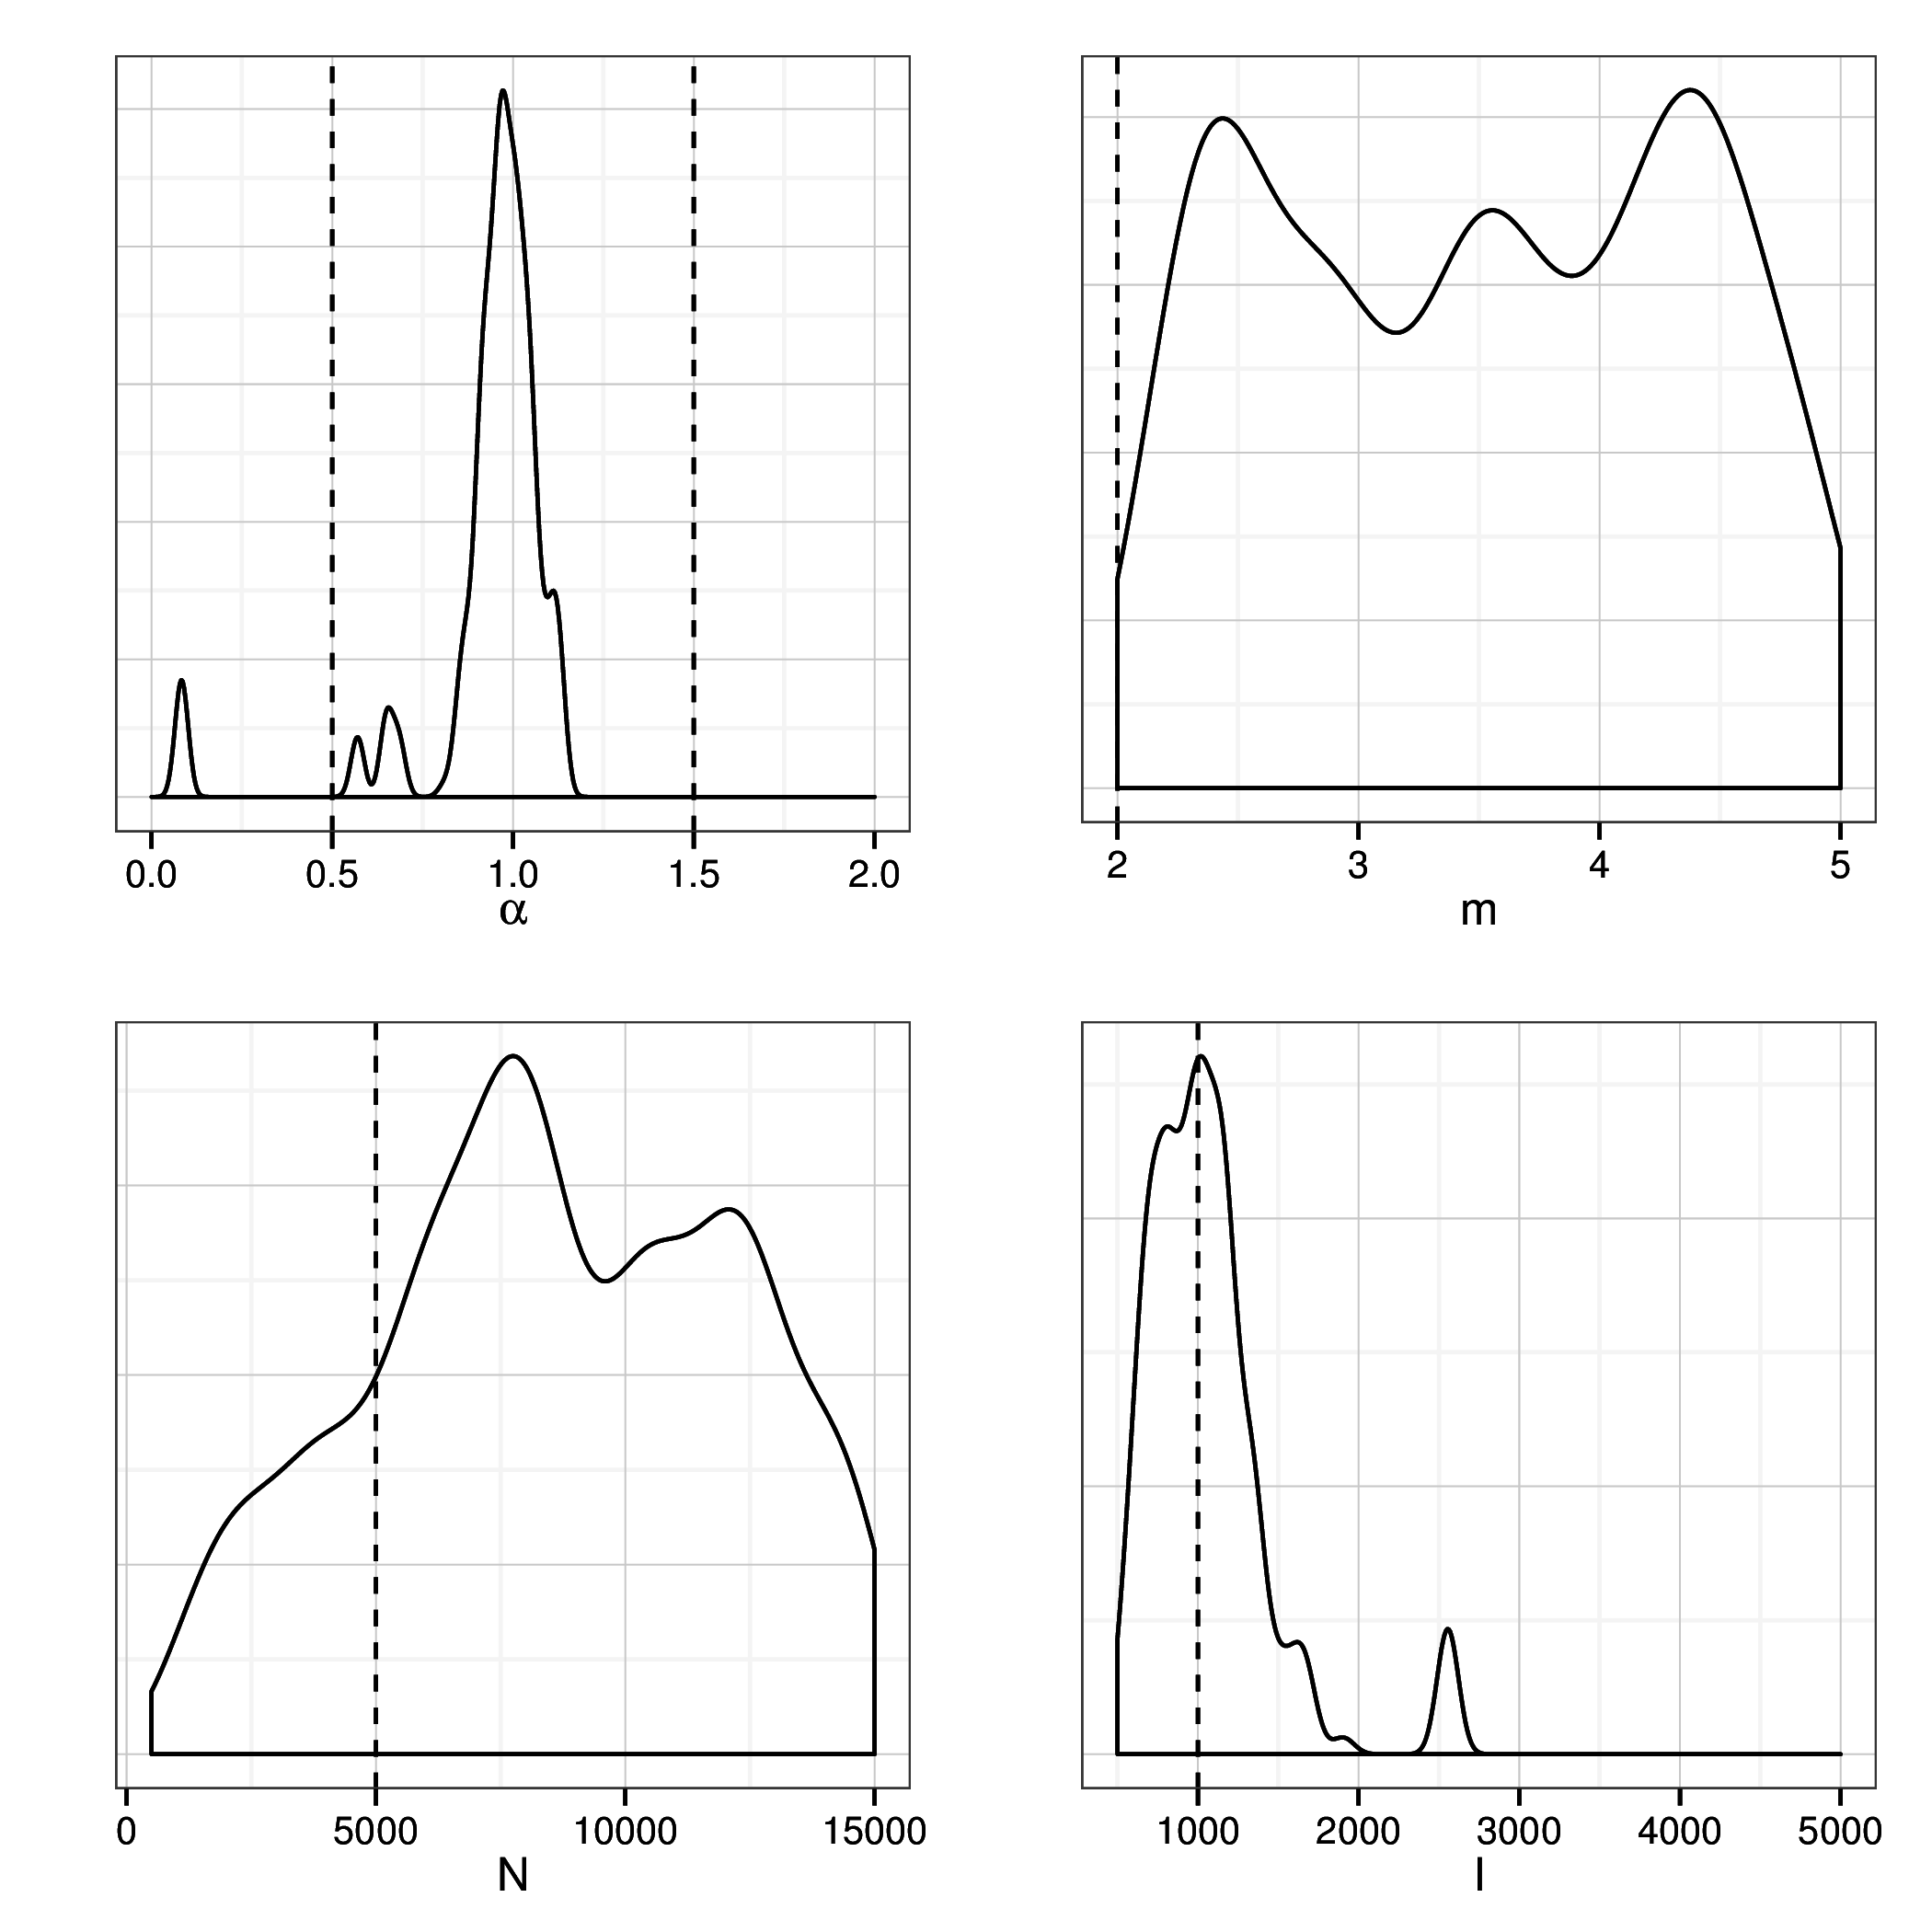
\includegraphics[scale=0.15]{mixed-alpha}

\subsection*{Realistic values of $\alpha$, as defined by $\gamma$}

The degree distributions of preferential attachment networks follow a power
law, meaning that the number of nodes of degree $k$ is proportional to
$k^\gamma$ for some $\gamma$ which is determined by $\alpha$. I looked at how
$\gamma$ varies with $\alpha$. Judging by this plot, we should upper bound
$\alpha$ at around 1.3 to 1.4. This is a nice result, since the posterior
density for values above 1.3 seems to always be zero (see eg. the above
$\alpha$ density), even though we put a uniform prior between 0 and 2.

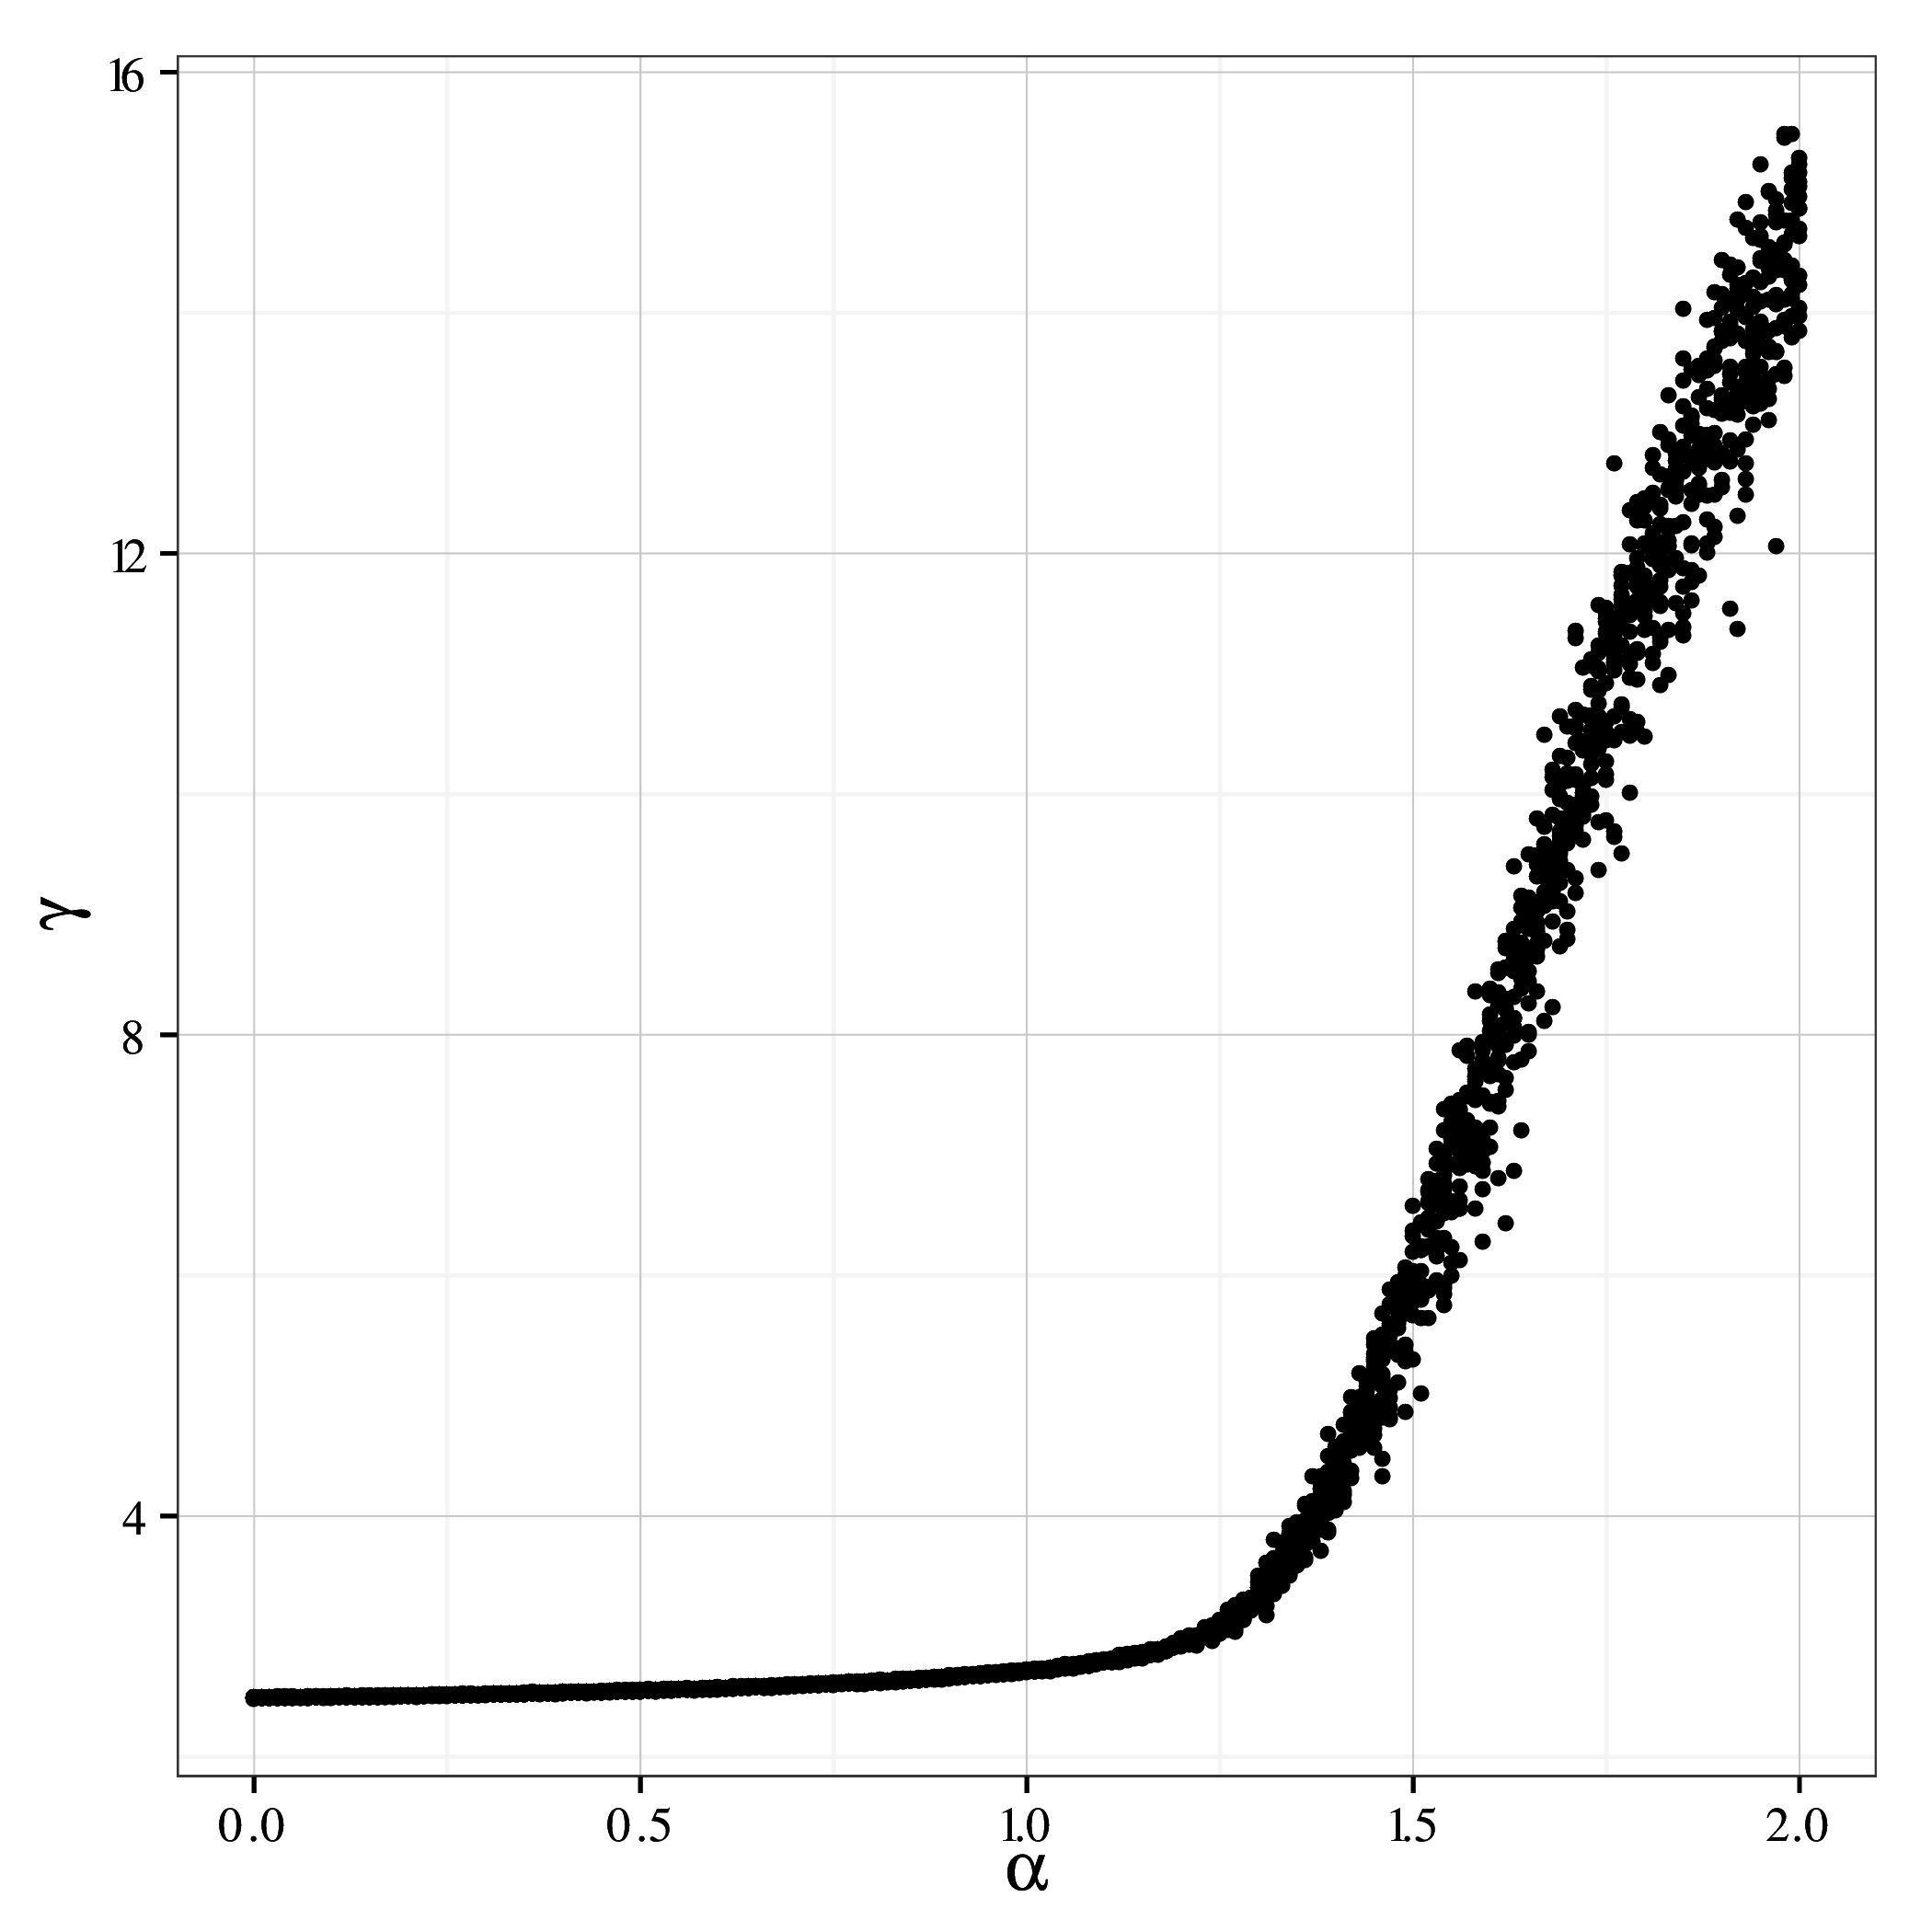
\includegraphics[scale=0.15]{gamma-alpha}

Relatedly, I will plot the estimated vs. actual values of $\gamma$ in addition
to $\alpha$.

\subsection*{Lineages-through-time as a standalone classifier}

I had previously evaluated combining nLTT with the tree kernel and found that
it brought down the accuracy of the classifier. I also looked at nLTT by itself,
and it's even worse than Sackin's index (see below).

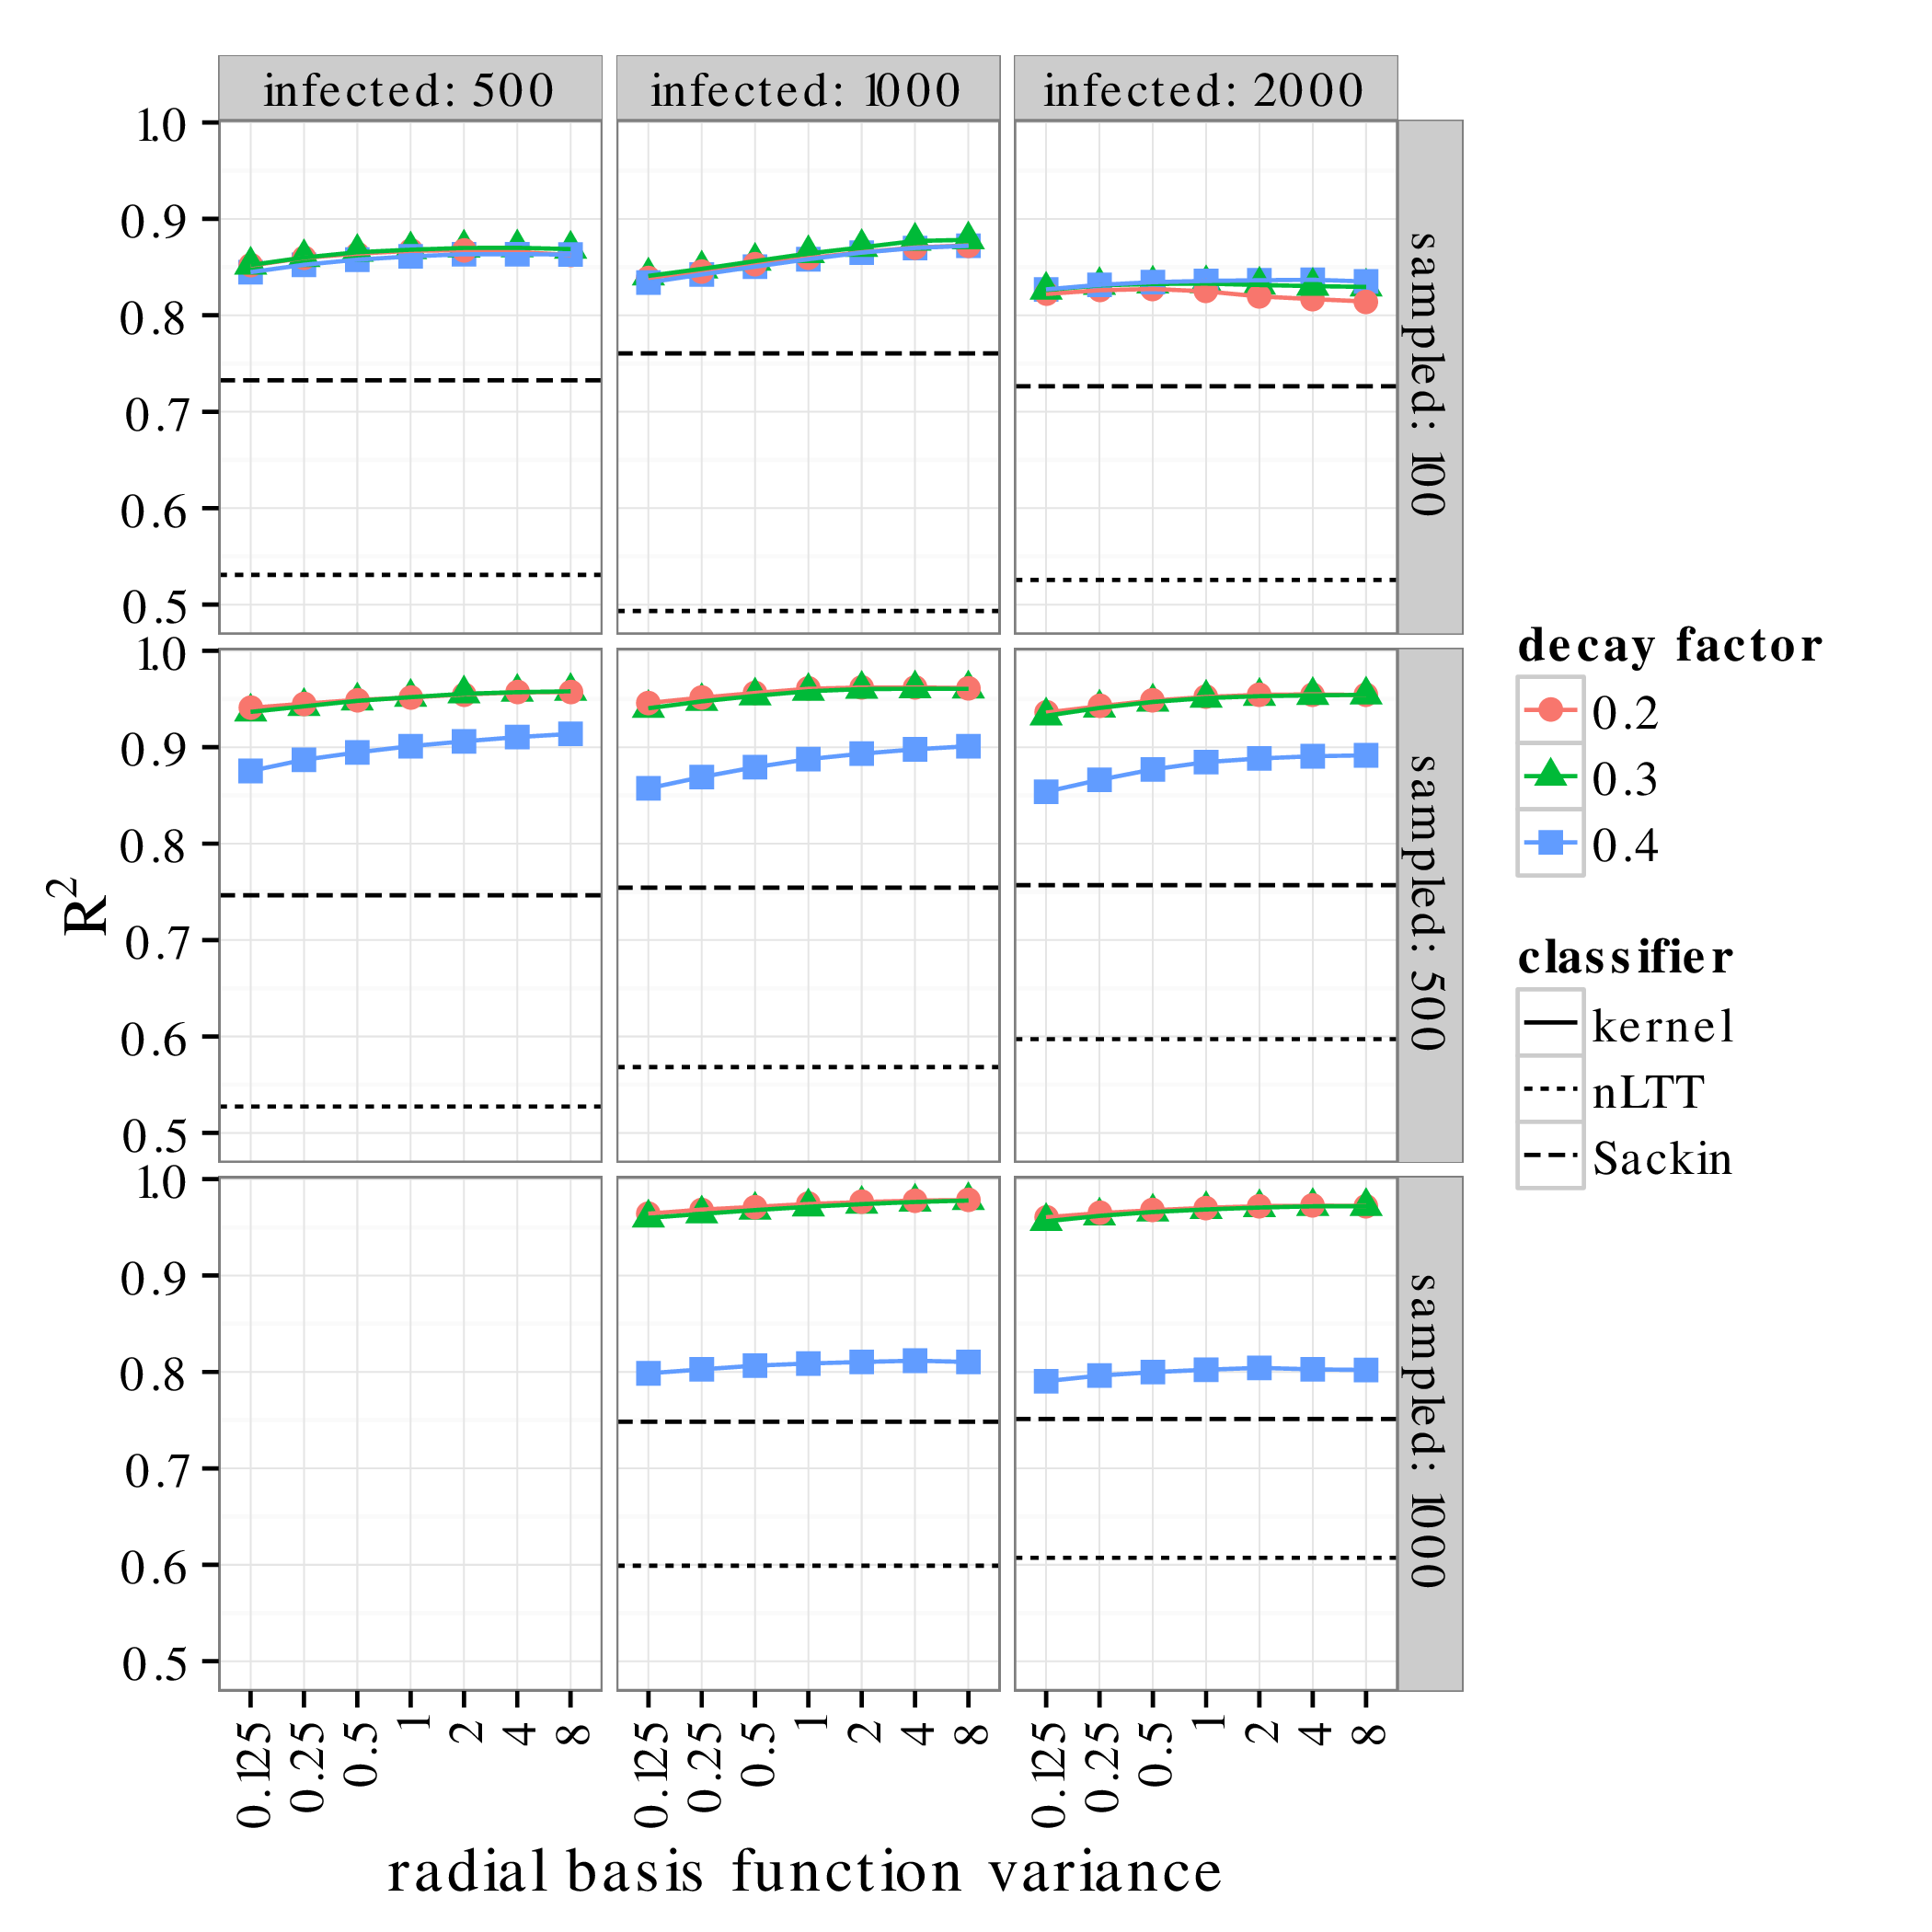
\includegraphics[scale=0.15]{crossv}

\subsection*{Expanded priors, free $m$}

We discussed expanding the prior regions so that the ``true'' values were less
in the middle, and also of allowing the $m$ parameter to be free in all
analyses. These updates are in progress. A bit of a preview is contained in the
first figure in this document, which shows that most of the posterior mass on
$I$ (the number of infected nodes) is concentrated around the true value on the
low end of the prior.

\subsection*{Biased sampling}

It was brought up that the assumption of random sampling from the population
might bias the results. I will evaluate the effect of non-random sampling based
on whether or not any of one's peers have been sampled. I have discussed an
implementation strategy with Art and will incorporate it into the program soon.

\subsection*{New real data}

For additional real-world use, as well as to circumvent possible privacy issues
with locally produced data, I am looking for more real-world data sets to which
I can apply the method. The best would be datasets which originate from known
phylogenetic clusters or epidemiologically linked patients. I have identified
the following one which describes their sample as a ``deeply sampled
subnetwork''.

\begin{quote}
Wang, Xicheng, et al. ``Targeting HIV Prevention Based on Molecular
Epidemiology Among Deeply Sampled Subnetworks of Men Who Have Sex With Men.''
Clinical Infectious Diseases (2015): civ526.
\end{quote}

I'm still on the lookout for others.

\subsection*{Literature support for the approach}

I need to put more effort into justifying why I'm doing this and why it's
important, such as the search for superspreader dynamics. Also, I would like to
emphasize a bit more that this is a general approach for fitting contact
network models to phylogenies, and is not restricted to this $\alpha$
parameter. I just happen to be using it because it is a simple and well-known
model, but is more realistic than the random graph model. Making this clearer
would (I hope) expand the potential utility of the method.

\end{document}
